\documentclass[12pt, a4paper]{article}
\usepackage[utf8]{inputenc}
\usepackage[russian]{babel}
\usepackage{extsizes}
\usepackage{mathtext}
\usepackage{hyperref}
\usepackage{amsmath}
\usepackage{amsfonts}
\usepackage{mathtools}
\usepackage{float}
\usepackage{subfig}
\usepackage[T2A]{fontenc}
\usepackage{graphicx}
\usepackage{algorithm}% http://ctan.org/pkg/algorithms
\captionsetup[algorithm]{labelformat=empty}
\usepackage[noend]{algpseudocode}

\begin{document}
    \begin{center}
        \textbf{ОПТИМИЗАЦИОННЫЙ АЛГОРИТМ РЕШЕНИЯ ОБРАТНОЙ ЗАДАЧИ СЛОЖНОГО ТЕПЛООБМЕНА}
    \end{center}
    \section{Введение}\label{sec:intro}
Стационарный радиационный и диффузионный теплообмен в ограниченной области
$\Omega \subset \mathbb{R}^3$ с границей $\Gamma = \partial \Omega$ моделируется в рамках  $P_1$--приближения для уравнения
переноса излучения следующей системой эллиптических уравнений~\cite{Pinnau07, AMC-13, Kovt14-1}:
\begin{equation}
    \label{eq:model}
    - a \Delta\theta + b\kappa_a(|\theta|\theta^3- \varphi)=0,   \quad
    - \alpha \Delta \varphi + \kappa_a(\varphi-|\theta|\theta^3)=0,\; x\in\Omega.
\end{equation}
Здесь $\theta$ -- нормализованная температура, $\varphi$ -- нормализованная интенсивность излучения,
усредненная по всем направлениям.
Положительные физические параметры $a$, $b$, $\kappa_a$ и $\alpha$, описывающие
свойства среды, определяются стандартным образом~\cite{Kovt14-1}.
Подробный теоретический и численный анализ различных постановок краевых и обратных задач,
а также задач управления для уравнений радиационного теплообмена
в рамках $P_1$--приближения для уравнения переноса излучения представлен в~\cite{Pinnau07}--\cite{CMMP20}.
Отметим также серьезный анализ интересных краевых задач, связанных с радиационным теплообменом,
представленный в~\cite{Amosov05}--\cite{Amosov20}.

Для постановки граничных условий нам потребуется разбить границу области на два участка
$\Gamma \coloneqq \partial \Omega =\overline{\Gamma}_1 \cup \overline{\Gamma}_2$,
где части границы не имеют пересечений.

Определим следующие функции
\begin{equation}
    \label{eq:boundary}
    \begin{aligned}
        \Gamma_1 :\; &\partial_n \theta = q_b, \; \theta = \theta_b, \\
        &\alpha\partial_n\varphi + \gamma (\varphi - \theta_b ^4 ) = 0, \\
        \Gamma_2 :\; & \partial_n \theta = q_b.
    \end{aligned}
\end{equation}
Далее введём следующее обозначение:

\[
    r \coloneqq \alpha \partial_n \varphi \text{ на }\Gamma_2, \\
    \tilde{r} \coloneqq \alpha \partial_n \varphi \text{ на }\Gamma_1.
\]

Обратная задача состоит в отыскании тройки функций $r \in  \Gamma_1, \{\theta, \varphi\} \in \Omega $
удовлетворяющих условиям~\eqref{eq:model}--\eqref{eq:boundary}, а также дополнительному условию
на участке границы $\Gamma_2$:
\begin{equation}
    \label{eq:boundary-extra}
    \theta = \theta_b \text{ на } \Gamma_2.
\end{equation}
Обратная задача~\eqref{eq:model}--\eqref{eq:boundary-extra} сводится к экстремальной задаче,
состоящей в минимизации функционала
\begin{equation}
    \label{eq:cost}
    J(\theta) = \frac{1}{2}\int\limits_\Gamma (\theta - \theta_b)^{2} d\Gamma \rightarrow \inf
\end{equation}
на решениях краевой задачи~\eqref{eq:model}--\eqref{eq:boundary}.


Альтернативным подходом может быть сведение исходной задачи к поиску некоторой
переменной $\psi = a\theta + \alpha b \varphi$:
\begin{equation}
    \label{eq:equation}
    - a \Delta \theta + g (\theta) = \frac{\kappa}{\alpha}\psi, \quad
    \Delta \psi = 0.
\end{equation}
С граничными условиями для температурного поля $\theta$ из~\eqref{eq:boundary},
дополненными следующими условиями для переменной $\psi$:
\begin{equation}
    \label{eq:boundary-2}
    \begin{aligned}
        \Gamma_1 &: \; \alpha \partial_n \psi + \gamma \psi = \alpha b \gamma \theta_b^4
        + \alpha a \theta_b + \gamma a q_b = r, \\
        \Gamma_2 &: \; \partial_n \psi = u.
    \end{aligned}
\end{equation}
Здесь $g(\theta) = b \kappa|\theta|\theta^3 + \frac{a\kappa}{\alpha}\theta$.
Функция $u$, в свою очередь неизвестна и играет роль управления.

В таком случае полученные далее дифференциальные уравнения являются независимыми и
могут считаться последовательно,
что отличается от классического подхода и может иметь высокий исследовательский потенциал.

Статья организована следующим образом.
В разд \. 2 вводятся необходимые пространства и операторы,
а также формальная постановка задачи оптимального управления.
Априорные оценки решения задачи \eqref{eq:model}--\eqref{eq:boundary-2}, на основе которых доказана разрешимость
указанной краевой задачи и задачи оптимального управления (1),(4),(5), получены в разд\. 3.
В разд \. 4 представлен алгоритм решения задачи управления, работа которого
проиллюстрирована численными примерами.

    \section{Формализация задачи управления}\label{sec:formalization}
Будем далее считать, что $\Omega \subset R$ - ограниченная строго липшицева область,
граница $\Gamma \equiv \partial \Omega$ состоит из конечного числа гладких кусков.
Будем предполагать, что для области $\Omega$ справедливы свойства 1, 2 из~\cite{}
Через $L^p, \; 1 \leq p \leq \infty$ обозначим пространство Лебега, через $H^s$ - пространство Соболева $W^s_2$.
$H^s_0(\Omega)$ есть замыкание $C^\infty_0(\Omega)$ по норме пространства $H^s(\Omega)$.
Далее через $(\dot, \dot), \; \| \dot \|$ обозначаем скалярное произведение и норму в $L^2(\Omega)$
\[
    (f, g) = \int_\Omega f(x)g(x)dx, \; \| f \| = (f, f).
\]
Пусть $V = H^2_0(\Omega)$.
Условия на область $\Omega$ позволяют выбрать скалярное произведение в V в виде
$[u, v] = (\nabla u, \nabla v), \| f \|_V = \| \nabla f \|$.
Через $U$ обозначаем пространство $L^2(\Gamma)$ с нормой
$\|u\|_\Gamma=\left(\int_\Gamma u^2 d\Gamma\right)^{1/2}.$

Будем предполагать, что

$(i) \;\; a,b,\alpha,\kappa_a, \lambda =\textrm{Const} > 0 ,$
$(ii) \;\, \theta_b, \,g \, u \in U,\;\; r=a(\theta_b+q_b).$


Определим операторы $A_1\colon V \to V'$, $A_2\colon U \to V'$, используя
следующие равенства, справедливые для любых $y,z \in V$, $w\in U$:
\[
    (A_1 y,z) = a(\nabla y, \nabla z) + \int_{\Gamma_1} yz d\Gamma, \,
    (A_2 y, z) = \alpha (\nabla y, \nabla z) + \int_{\Gamma_1} \gamma yz d\Gamma.
\]
    {\it Слабым решением} задачи~\eqref{model}-\eqref{boundary} будем называть
пару $\theta, \psi \in V$ если
\begin{equation}
    \label{weak}
    A_1\theta  + g(\theta) = \frac{\kappa}{\alpha} \psi + f_1, \quad
    A_2\psi = f_2 + B_2 u.
\end{equation}

Здесь
$(f_1, v) = \int_{\Gamma_1} (a q_b + \theta_b)d\Gamma + \int_{\Gamma_2} a q_b d\Gamma$,\\
$(f_2, v) = \int_{\Gamma_1} r v d\Gamma$,\\
$(B_1 h,v) = \int_{\Gamma_1} h v d\Gamma$,\\
$(B_2 u, v) = \int_{\Gamma_2} u v d\Gamma$,\\
$g(\theta) = b\kappa_a \theta^3 |\theta| + \frac{a\kappa_a}{\alpha}\theta.$



    \section{Вывод системы оптимальности}\label{sec:optimality}
Лагранжиан задачи выглядит следующим образом:
\begin{equation}
    \label{eq:lagrange}
    L = J_\lambda + (A_1 \theta+ g(\theta) - \frac{\kappa}{\alpha}\psi -f_1, p_1)
    + (A_2 \psi - f_2 - B_2 u, p_2).
\end{equation}
\begin{equation}
    \label{eq:lagrange_t}
    <L'_\theta, v> = (\theta - \theta_b, v)_{\Gamma_1}
    + (A_1 v + g'(\theta)v, p_1) = 0.\, \forall v \in V.
\end{equation}
Здесь
\[
    g'(\theta) = 4 b \kappa |\theta |^ 3 + \frac{a \kappa}{\alpha}  > 0.
\]
Таким образом получаем, что
\begin{equation}
    \label{eq:a1}
    A_1 p_1 + g'(\theta) p_1 = - B_1(\theta - \theta_b).
\end{equation}

\begin{equation}
    \label{eq:lagrange_p}
    <L'_\psi, v> = - ( \frac{\kappa}{\alpha} v, p_1) + (A_2v, p_2) = 0.
\end{equation}
\begin{equation}
    \label{eq:a2}
    A_2 p_2 - \frac{\kappa}{\alpha} p_1 = 0.
\end{equation}

\begin{equation}
    \label{eq:lagrange_u}
    <L'_u, w> = \lambda(u, w)_{\Gamma_2} - (B_2 w, p_2) = 0.
\end{equation}

Из последнего уравнения естественным образом следует
\begin{equation}
    \label{eq:a3}
    \lambda u = p_2 \text{ на } \Gamma_2.
\end{equation}


    \section{Алгоритм решения задачи и численные примеры}\label{sec:experiments}
Представим алгоритм решения задачи управления.
В соответствии с~\eqref{eq:model} градиент функционала качества равен
\[
    J'_\lambda (u) = \lambda u - p_2.
\]
Здесь $u\in U$ -- управление в граничном условии~\eqref{eq:boundary-psi-3}, $p_2$ -- соответствующая компонента
сопряженного состояния из системы~\eqref{eq:model}--\eqref{eq:model}.

Предлагаемый алгоритм решения задачи (CP) выглядит следующим образом.
\begin{algorithm}[H]
    \caption{Алгоритм градиентного спуска}
    \begin{algorithmic}[1]
        \State Выбираем значение градиентного шага $\varepsilon$,
        \State Выбираем количество итераций $N$,
        \State Выбираем начальное приближение для управления $u_0 \in U$,
        \For{$k \gets 0,1,2,\dots,N$}
            :
            \State Для $u_k$ рассчитываем состояние $ y_k = \{\theta_k, \psi_k\} $ --
            решение задачи~\eqref{eq:model-psi},\eqref{eq:boundary-psi-2},\eqref{eq:boundary-psi-3}.
            \State Рассчитываем значение функционала качества $J_\lambda(\theta_k, u_k)$.
            \State Рассчитываем сопряженное состояние $p_k=\{p_{1k},p_{2k}\}$ из
            уравнений~\eqref{eq:conjugate_1},\eqref{eq:conjugate_2},
            где $ \hat{\theta} := \theta_k, \hat{u}=u_k$.
            \State Пересчитываем управление $u_{k+1} = u_k - \varepsilon (\lambda u_k - p_2)$
        \EndFor
    \end{algorithmic}\label{alg:algorithm}
\end{algorithm}

Значение параметра $\varepsilon$ выбирается эмпирически таким образом, чтобы значение
$\varepsilon (\lambda u_k - p_2)$ являлось существенной поправкой для $u_{k+1}$.
Количество итераций $N$ выбирается достаточным для выполнения условия
$J_\lambda(\theta_k, u_k) - J_\lambda(\theta_{k+1}, u_{k+1}) < \delta$, где $\delta>0$ определяет точность расчетов.

Примеры, рассмотренные ниже, иллюстрируют работоспособность предложенного алгоритма при
малых значениях параметра регуляризации $\lambda \leq 10^{-12}$.
В первом примере выполнены тестовые расчеты для куба.

Отметим, что для численного решения прямой задачи с заданным
управлением использовалась слабая формулировка
и метод Ньютона для линеаризации задачи.
Решение сопряженной системы, которая является линейной при
заданной температуре, не вызывает трудностей.
Для численного моделирования использовался солвер FEniCS~\cite{fenics, dolfin}.

\textbf{Пример 1.}
Приведем примеры расчетов для куба
\[
    \Omega = {(x, y, z), 0 \leq x,y,z \leq l}.
\]
Границу куба разобьём на два участка:
\[
    \Gamma_1 = \{(x, y, z), 0 \leq x,y, \leq l, z \in 0, l\}, \;
    \Gamma_2 = \partial \Omega \setminus \hat{\Gamma_1}.
\]

Будем считать, что $l=1~\text{см}$, $a = 0.006[\text{см}^2/\text{c}]$,
$b=0.025[\text{см}/\text{с}]$,
$\kappa_a=1[\text{см}^{-1}]$, $\alpha = 0.(3)[\text{см}]$.
Указанные параметры соответствуют стеклу~\cite{Grenkin5}.
Параметр регуляризации $\lambda=10^{-12}$.

Пусть граничные данные имеют следующий вид:
\begin{gather*}
    q_b = 0.5, \quad
    \theta_b = 0.1 + z/2, \quad
    \psi_0 = 0.1.
\end{gather*}
Применяя алгоритм градиентного спуска
с начальным приближением $u_0 = 0.1$, находим приближенное решение
$\{\theta_\lambda,\varphi_\lambda,u_\lambda\}$ задачи (CP)\@.
Для демонстрации того, что алгоритм находит приближенное решение задачи с данными
Коши для температуры, важно сравнить значения $\partial_n\theta_\lambda$ на $\Gamma$ с $q_b$.

На рисунке~\ref{fig:img_test_1} представлены изолинии модуля относительной разности
$|\partial_n\theta_\lambda-\theta_n|/\ \theta_n$
на грани куба в плоскости $z=0$, где
$\partial_n\theta_\lambda=\partial\theta_\lambda/\partial z$,
а также динамика функционала качества, определяющего
норму разности $\|\theta_\lambda -\theta_b\|^2_U$.
На остальных гранях куба значения имеют тот же порядок малости.

\begin{figure}[H]
    \centering
    \subfloat[$|\partial_n \theta_\lambda - q_n|/\ q_n$]
    {
        \label{fig:img_test_1}
        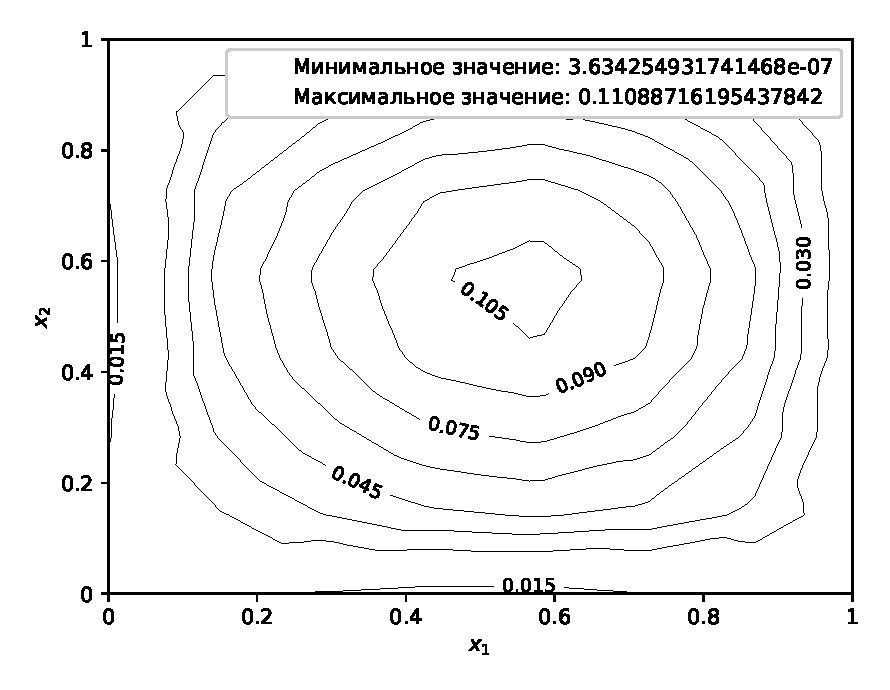
\includegraphics[width=.49\linewidth]{img/exp1_iso}
    }
    \subfloat[Изменение функционала качества по итерациям]
    {
        \label{fig:quality_1}
        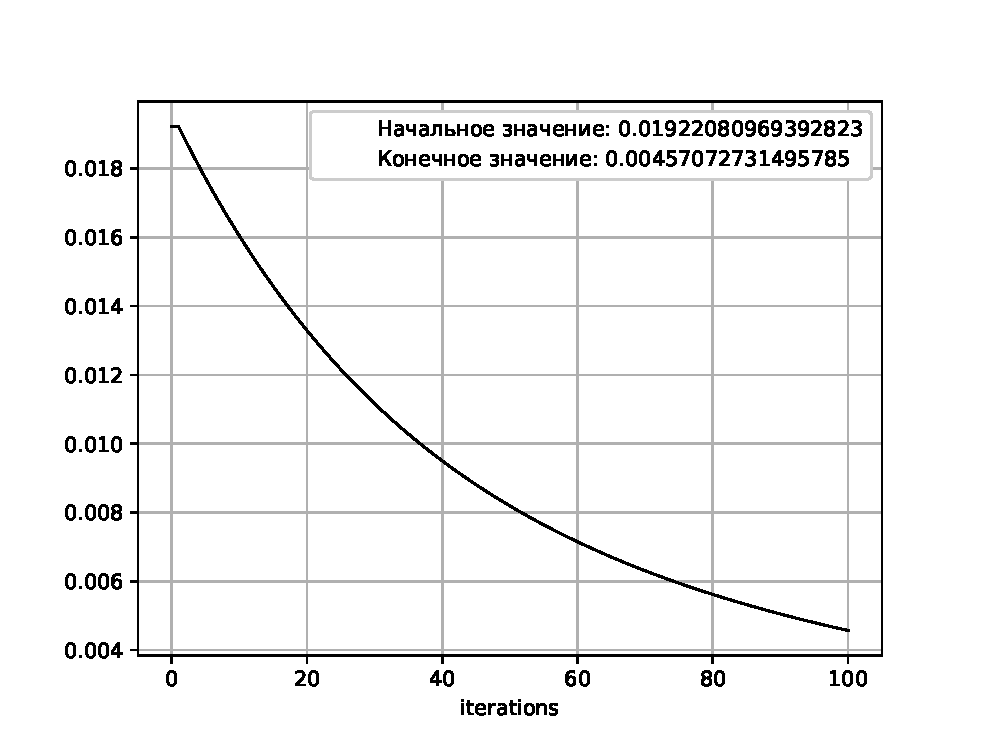
\includegraphics[width=.49\linewidth]{img/exp1_quality}
    }
    \caption{Результаты первого эксперимента}
    \label{fig:1}
\end{figure}


\textbf{Пример 2.}
Рассмотрим единичный куб, Из которого  вырезан шар $T$ c центром в точке $c = \{\| t - c \| < 0.2\}$,
$T = \{/\ t, \|t - c \| \}$.
$\Omega = \{(x,y,z),  0 \leq x,y,z \leq 1 \} /\ T$.
Внешнюю границу куба мы обозначим за $\Gamma_1$, границу шара обозначим за $\Gamma_2$.
Граничные условия положим следующими:
\begin{gather*}
    q_b = 0.5, \quad
    \theta_b = 0.1 + z/2, \quad
    \psi_0 = 0.1.
\end{gather*}

\begin{figure}[H]
    \centering
    \subfloat[$\theta_\lambda$ по вертикальному, центральному срезу]
    {
        \label{fig:exp2_theta_end}
        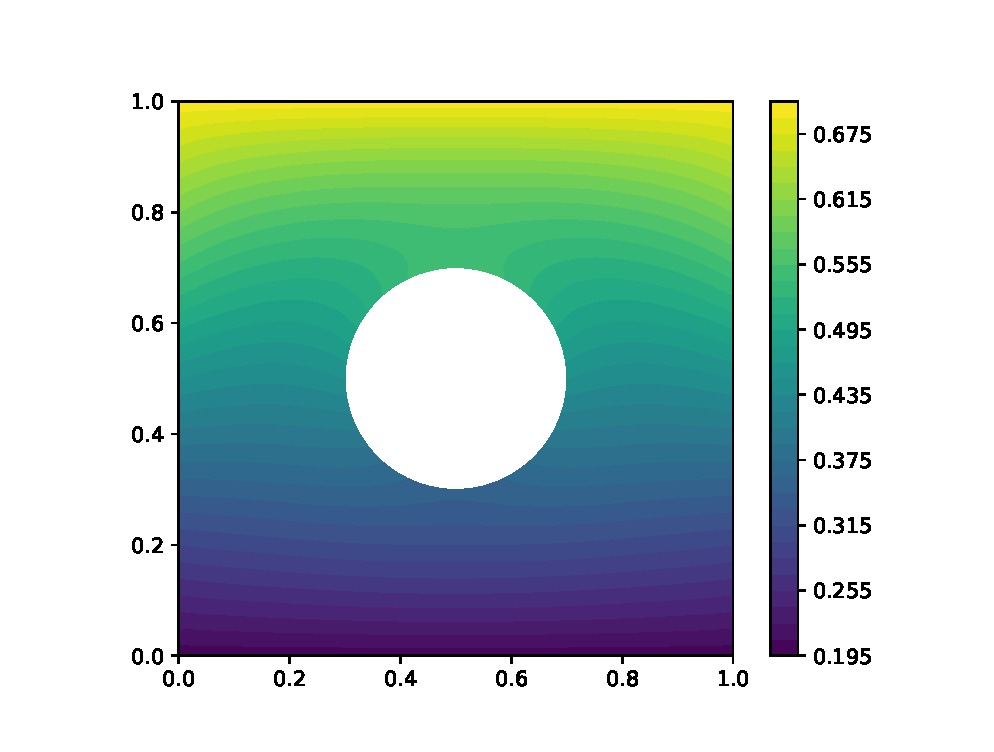
\includegraphics[width=.49\linewidth]{img/exp2_theta_end}
    }
    \subfloat[Изменение функционала качества по итерациям]
    {
        \label{fig:exp2_quality}
        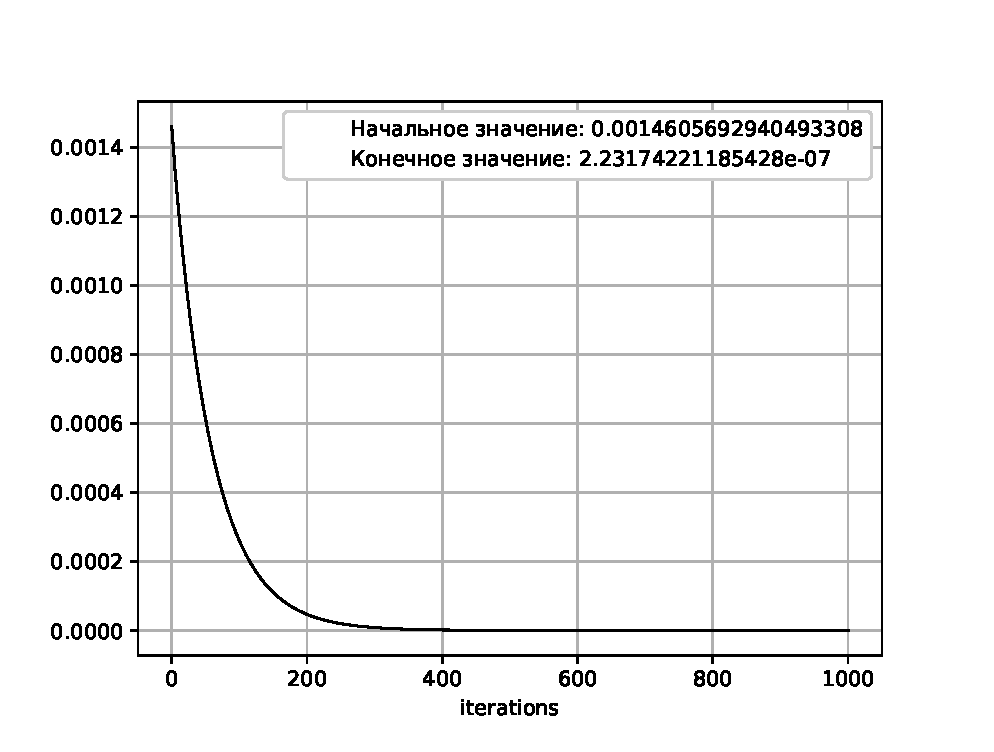
\includegraphics[width=.49\linewidth]{img/exp2_quality}
    }
    \caption{Результаты первого эксперимента}
    \label{fig:2}
\end{figure}
    %! Suppress = LineBreak
\begin{thebibliography}{999}

    \bibitem{Pinnau07}
    Pinnau R. Analysis of optimal boundary control for radiative heat transfer modeled by $SP_1$-system //
    Commun. Math. Sci. 2007. V. 5. \textnumero~4. P. 951--969.

    \bibitem{AMC-13}
    Kovtanyuk A.E., Chebotarev A.Yu. An iterative method for solving a complex heat transfer problem // Appl. Math. Comput. 2013. V. 219. \textnumero~17. P. 9356--9362.
    \bibitem{Kovt14-1}
    Kovtanyuk A.E., Chebotarev A.Yu., Botkin N.D., Hoffmann K.-H. The unique solvability of a complex 3D heat transfer problem // J. Math. Anal. Appl. 2014. V. 409. \textnumero~2. P. 808--815.
    \bibitem{JVM-14}
    Ковтанюк А.Е., Чеботарев А.Ю. Стационарная задача сложного теплообмена // Ж. вычисл. матем. и матем. физ. 2014. Т. 54. \textnumero~4. С. 711--719.
    \bibitem{Kovt14-2}
    Ковтанюк А.Е., Чеботарев А.Ю. Стационарная задача свободной конвекции с радиационным теплообменом // Дифференц. ур-ния. 2014. Т. 50. \textnumero~12. С. 1590--1597.
    \bibitem{Kovt14-3}
    Kovtanyuk A.E., Chebotarev A.Yu., Botkin N.D., Hoffmann K.-H. Theoretical analysis of an optimal control problem of conductive-convective-radiative heat transfer // J. Math. Anal.
    Appl. 2014. V. 412. \textnumero~1. P. 520--528.
    \bibitem{Grenkin1}
    Гренкин Г.В., Чеботарев А.Ю. Нестационарная задача сложного теплообмена // Ж. вычисл. матем. и матем. физ. 2014. Т. 54. \textnumero~11. С. 1806--1816.
    \bibitem{CNSNS-15}
    Kovtanyuk A.E., Chebotarev A.Yu., Botkin N.D., Hoffmann K.-H. Unique solvability of a steady-state complex heat transfer model // Commun. Nonlinear Sci. Numer. Simul. 2015. V. 20. \textnumero~3. P. 776--784.

    \bibitem{Grenkin3}
    Гренкин Г.В., Чеботарев А.Ю. Неоднородная нестационарная задача сложного теплообмена // Сиб. электрон. матем. изв. 2015. Т. 12. С. 562--576.
    \bibitem{Grenkin4}
    Гренкин Г.В., Чеботарев А.Ю. Нестационарная задача свободной конвекции с радиационным теплообменом // Ж. вычисл. матем. и матем. физ. 2016. Т. 56. \textnumero~2. С. 275--282.
    \bibitem{Grenkin5}
    Grenkin G.V., Chebotarev A.Yu., Kovtanyuk A.E., Botkin N.D., Hoffmann K.-H. Boundary optimal control problem of complex heat transfer model // J. Math. Anal. Appl. 2016. V. 433. \textnumero~2. P. 1243--1260.



    \bibitem{JMAA-16}
    Kovtanyuk A.E., Chebotarev A.Yu., Botkin N.D., Hoffmann K.-H. Optimal boundary control of a steady-state heat transfer model accounting for radiative effects // J. Math. Anal. Appl.
    2016. V. 439. \textnumero~2. P. 678--689.
    \bibitem{AMC-16}
    Chebotarev A.Yu., Kovtanyuk A.E., Grenkin G.V., Botkin N.D., Hoffmann K.-H\@.
    Nondegeneracy of optimality conditions in control problems for a radiative-conductive heat transfer model // Appl. Math. Comput. 2016. V. 289. P. 371--380.
    \bibitem{JVM-16}
    Ковтанюк А.Е., Чеботарев А.Ю. Нелокальная однозначная разрешимость стационарной задачи сложного теплообмена // Ж. вычисл. матем. и матем. физ. 2016. Т. 56. \textnumero~5. С. 816--823.
    \bibitem{ESAIM}
    Chebotarev A.Yu., Grenkin G.V., Kovtanyuk A.E. Inhomogeneous steady-state problem of complex heat transfer // ESAIM Math. Model. Numer. Anal. 2017. V. 51. \textnumero~6. P. 2511--2519.

    \bibitem{CNSNS18}
    Chebotarev, A.Y., Grenkin, G.V., Kovtanyuk, A.E., Botkin, N.D., Hoffmann, K.-H. Diffusion approximation of the radiative-conductive heat transfer model with Fresnel matching conditions// Communications in Nonlinear Science and Numerical Simulation. 57 (2018) 290-298.

    \bibitem{JMAA-18}
    Chebotarev A.Yu., Grenkin G.V., Kovtanyuk A.E., Botkin N.D., Hoffmann K.-H. Inverse problem with finite overdetermination for steady-state equations of radiative heat exchange // J. Math. Anal. Appl. 2018. V. 460. \textnumero~2. P. 737--744.
    \bibitem{JMAA-19}
    Chebotarev A.Yu., Pinnau R. An inverse problem for a quasi-static approximate model of radiative heat transfer // J. Math. Anal. Appl. 2019. V. 472. \textnumero~1. P. 314--327.
    \bibitem{JVM-19-INV} Гренкин Г.В., Чеботарев А.Ю. Обратная задача для уравнений сложного теплообмена // Журнал вычислительной математики и математической физики. 2019, том 59, N 8, с. 1420-1430.

    \bibitem{CNSNS19}
    Chebotarev A.Y., Kovtanyuk A.E., Botkin N.D. Problem of radiation heat exchange with boundary conditions of the Cauchy type // Communications in Nonlinear Science and Numerical Simulation. 75 (2019) 262-269.

    \bibitem{CMMP20}
    Колобов А.Г., Пак Т.В., Чеботарев А.Ю.
    Стационарная задача радиационного теплообмена с граничными условиями типа Коши
    // Журнал вычислительной математики и математической физики.
    2019, том 59, N 7, с. 1258--1263.

    \bibitem{Amosov05}
    Амосов~А.А. Глобальная разрешимость одной нелинейной
    нестационарной задачи с нелокальным краевым условием типа
    теплообмена излучением~// Дифференц. ур-ния. Т.~41. N~1.
    2005. С.~93--104.

    \bibitem{Amosov10}
    Amosov~A.A. Stationary nonlinear nonlocal problem of
    radiative-conductive heat transfer in a system of opaque bodies
    with properties depending on the radiation frequency~// J\@.
    Math. Sc. 2010. V.~164. N~3. P.~309--344.

    \bibitem{Amosov16}
    Amosov A. Unique Solvability of a Nonstationary Problem of Radiative - Conductive
    Heat Exchange in a System of Semitransparent Bodies // Russian J. of Math.
    Phys. 2016. V. 23, N~3. P.~309-334.

    \bibitem{Amosov17}
    Amosov A.A. Unique Solvability of Stationary Radiative - Conductive Heat Transfer
    Problem in a System of Semitransparent Bodies // J. of Math. Sc.(United
    States). 2017. V. 224. N~5. P.~618-646.

    \bibitem{Amosov20-1}
    Amosov, A.A. Asymptotic Behavior of a Solution to the Radiative Transfer Equation in a Multilayered Medium with Diffuse Reflection and Refraction Conditions // J Math Sci 244, 541-575 (2020).

    \bibitem{Amosov20}
    Amosov A.A., Krymov N.E. On a Nonstandard Boundary Value Problem Arising in Homogenization of Complex Heat Transfer Problems // J. of Math. Sc.(United
    States). 2020. V. 244. P.~357 - 377.




    \bibitem{Kufner} S.~Fu\v{c}ik, A.~Kufner, Nonlinear differential equations,
    Elsevier, Amsterdam--Oxford--New York, 1980.

    \bibitem{10} A.V.~Fursikov, Optimal Control of Distributed
    Systems. Theory and Applications, American Math. Soc., 2000.

    \bibitem{11} A.D.~Ioffe, V.M.~Tikhomirov, Theory of Extremal
    Problems, North-Holland, Amsterdam, 1979.

    \bibitem{fenics} M. S. Alnaes, J. Blechta, J. Hake, A. Johansson,
    B. Kehlet, A. Logg, C. Richardson, J. Ring, M. E. Rognes, G. N. Wells
    The FEniCS Project Version 1.5
    Archive of Numerical Software, vol. 3, 2015,

    \bibitem{dolfin} A. Logg and G. N. Wells, DOLFIN: Automated Finite Element Computing
    ACM Transactions on Mathematical Software, vol. 37, 2010

    \bibitem{mesenev-github} \url{https://github.com/mesenev/articles_src}


\end{thebibliography}

\end{document}
